%% 
%% Vorlesung <2012-12-14 Fri>, Fortsetzung
%% 

\chapter{Geod\"atische und die Exponentialabbildung}

\begin{emptythm}[Heuristik:] Geod"atische sind Minimalstellen des Energiefunktionals $\gamma \mapsto E(\gamma) = \int \|\dot\gamma\|^2$. 
  Was sind kritische Punkte dieser Abbildung?
  F"ur $f \in C^{\infty}(M)$ ist $p$ kritischer Punkt, wenn alle Richtungsableitungen verschwinden, das hei"st $0 = X(f) = \difffrac[t=0]{}{t}(f(c(t)))$.
\end{emptythm}

\begin{center}\begin{tikzpicture}[font=\scriptsize]
    %	\draw[step=0.25,gray!15] (-6,-4) grid (6,4); \draw[step=0.5,gray!30] (-6,-4) grid (6,4); \fill (0,0) circle(0.1); %Hilfsgitter
    
    \coordinate (p) at (-2,-1); \coordinate (q) at (2,1); \coordinate (wirbel) at (-0.5,-0.5); %die beiden Endpunkte und der Wendepunkt
    \coordinate (ctrl1) at (1,0); % Wendetangente
    \def\left{0.75} % linke Laenge der Wendetangente
      \def\right{1.75} % rechte Laenge
    \fill (p) circle(0.05)node[below]{$p$}; \fill (q) circle(0.05)node[right]{$q$};
    
    \draw[name path=kurve] (p) ..controls(p) and ($(wirbel) - \left*(ctrl1)$).. (wirbel)node[below]{$\gamma(t)$} ..controls($(wirbel) + \right*(ctrl1)$) and (q)..node[below]{$\gamma$} (q);
    \fill (wirbel) circle(0.05);
    
    \coordinate (vec) at (-0.5,1);
    \foreach \shift in {0.2,0.4,...,1}{
      \coordinate (neuwirbel) at ($(wirbel) + \shift*(vec)$);
      \draw[name path=obere kurve] (p) ..controls(p) and ($(neuwirbel) - \left*(ctrl1)$).. (neuwirbel) ..controls($(neuwirbel) + \right*(ctrl1)$) and (q).. (q);
    }
    \draw[->] (wirbel) -- ($(wirbel) + 1.3*(vec)$);
    
    \path[name path=vert] (0,-1) -- (0,1);
    \path[name intersections={of={kurve and vert}}];
    \fill (intersection-1) circle(0.05);
    \draw[->] (intersection-1) -- ($(intersection-1) + (0.5,1)$);
    \path[name intersections={of={obere kurve and vert}}];
    \node[above] at (intersection-1) {$h_s$};
  \end{tikzpicture}\end{center}

Eine \quot{Kurve} durch $\gamma$ ist eine sogenannte \CmMark[Variation!glatte]{glatte Variation} $h\colon[0,1]\times[0,1] \to M$, $h(s,t) = h_s(t)$ mit $h_0 = \gamma$ und $h_s(0) = p$, sowie $h_s(1) = q$ f"ur alle $s \in [0,1]$.
Dann ist
\begin{align*}
  X(t) = \difffrac[s=0]{}{s}h_s(t)
\end{align*}
ein glattes Vektorfeld entlang $\gamma$.
Ferner gilt $X(0) = 0$ und $X(1) = 0$.
Nun betrachte
\begin{align*}
  0  = \difffrac[s=0]{}{s}E(h_s) &= \int_{0}^{1} \difffrac[s=0]{}{s} \left<\difffrac{}{t} h_s(t),\difffrac{}{t}h_s(t)\right>\\
  & = \int_0^1 2 \left<\nabla_s \difffrac{}{t}h_s(t), \difffrac{}{t}h_s(t)\right>\\
  & = \int_0^1 2 \left<\nabla_t\smash{\underbrace{\difffrac{}{s}h_s(t)}_{=X(t)}}, \difffrac{}{t}h_s(t)\right> \vphantom{\underbrace{\difffrac{}{s}h_s(t)}_{=X(t)}}\\
  & = \int_0^1 2 \left<\nabla_tX,\difffrac{}{t}h_s(t)\right>\\
  & = 2 \int_0^1 \difffrac{}{t}\left<X,\difffrac{}{t}h_s(t)\right> - \left<X,\nabla_t\difffrac{}{t}h_s(t)\right>\\
  & = \underbrace{2 \int_0^1 \difffrac{}{t}\left<X,\difffrac{}{t}h_s(t)\right>}_{=0} - 2 \int_0^1 \left<X,\nabla_t\difffrac{}{t}h_s(t)\right>\\
  & = -2 \int_0^1 \left<X(t),\nabla_t\dot\gamma(t)\right>\dop t
\end{align*}

% Definition 8.1
\begin{Dfn}\label{dfn-8-1}
  Eine glatte Kurve $c$ in $M$ hei"st \CmMark{Geod\"atische}\footnote{Die "Aquivalenz zur bereits bekannten Definition wird in K"urze gezeigt.}, wenn $\nabla_t\dot c \equiv 0$ gilt.
\end{Dfn}

Ist $c$ Geod"atische, so ist $c$ proportional zur Bogenl"ange parametrisiert, das hei"st $\|\dot c\| = $const, denn $\difffrac{}{t}\|\dot c(t)\|^{2} = \difffrac{}{t}\left<\dot c(t),\dot c(t) \right> = 2\left<\nabla_t\dot c(t), \dot c(t)\right> = 0$.
Mit $c$ ist auch jede affine Umparametrisierung $t \mapsto c(at + b)$ eine Geod"atische.

% Proposition 8.2
\begin{Prop}
  F"ur jedes $p \in M$ und $v \in \T_pM$ existiert genau eine Geod"atische $\gamma_{p,v}\colon[0,\epsilon] \to M$ mit $\gamma_{p,v}(0) = p$ und $\dot \gamma_{p,v}(0) = v$.
  Zudem h"angt $\gamma_{p,v}$ glatt von $p$ und $v$ ab.
\end{Prop}

\begin{bew}
  \begin{enumerate}[label=(\Alph*),leftmargin=*,widest=B]
  \item Es sei $(\phi, U)$ eine Karte um $p$, $\gamma^i(t) = \phi^i(\gamma(t))$. Dann besitzt das folgende Anfangswertproblem
    \begin{align*}
      \begin{cases}
        0 = \nabla_t\dot \gamma|_t = \sum_k\left(\ddot \gamma^k(t) + \sum_{ij}\Gamma_{ij}^k\big(\gamma(t)\big)\dot \gamma^i(t)\gamma^j(t)\right) \pdifffrac[\gamma(t)]{}{x^k}\\
        \gamma^i(0) = \phi^i(p)\\
        \dot\gamma^i(0) = \xi_p^i, \quad v = \sum \xi^i_p\pdifffrac[p]{}{x^i}
      \end{cases}
    \end{align*}
    eine eindeutige L"osung (lokal), welche glatt von den Startwerten $p$ und $v$ abh"angt.
  \item (Alternativ) Ist $(\phi, U)$ eine Karte von $M$ um $p$, dann ist
    \[ \overline \phi \colon \left\{\begin{array}{cccl}
        \T M|_U &\to& \R^{2m}&\\
        X_p=\sum \xi_p^i\pdifffrac[p]{}{x^i} &\mapsto& \overline\phi(X_p) &= (\phi^1(p), \ldots, \phi^m(p), \xi_p^1, \ldots, \xi_p^m)\\
        &&& =: (y^1, \ldots, y^{2m})
      \end{array}\right.\]
    eine Karte von $\T M$.	
    Es sei $S$ das durch
    \[ S \colon \left\{ \begin{array}{ccc}
        \T M &\to& \T\T M\\
        X = \sum \xi^i \pdifffrac{}{x^i} &\mapsto& \sum_i^m \xi^i \pdifffrac{}{y^i} - \sum_{i,j,k=1}^{m} \Gamma_{ij}^k \xi^i\xi^j\pdifffrac{}{y^{m+k}}
      \end{array}\right.\]
    definierte glatte Vektorfeld auf $\T M$.	
    $g^t$ ist genau dann Integralkurve von $S$ durch $X_p = \sum \xi_p^i\pdifffrac[p]{}{x^i}$, wenn
    \begin{align*}
      \difffrac{}{t}g^t = \dot g^t = S(g^t) \text{ und } g^0 = X_p.
    \end{align*}
    Setzt man $\overline \phi(g^t) = (\gamma^1(t), \ldots, \gamma^m(t),\eta^1(t), \ldots, \eta^m(t))$, so ist dies genau dann der Fall, wenn gilt:
    \begin{align*}
      & (\dot\gamma^1,\ldots, \dot\gamma^m,\dot\eta^1,\ldots, \dot\eta^m) = \left(\eta^1, \ldots, \eta^m, -\sum_{i,j}\Gamma_{ij}^1\eta^i\eta^j, \ldots, -\sum_{i,j}\Gamma_{ij}^m\eta^i\eta^j\right)\\
      & \rightsquigarrow \eta^i = \dot\gamma^i \text{ und } \ddot\gamma = -\sum_{i,j}\Gamma_{ij}^k\dot\gamma^i \dot\gamma^j
    \end{align*}
    und 
    \begin{align*}
      (\gamma^1(0), \ldots, \gamma^m(0), \eta^1(0), \ldots, \eta^m(0) = \overline\phi(X_p) = (\phi^1(p), \ldots, \phi^m(p), \xi_p^1, \ldots, \xi_p^m)
    \end{align*}
    also genau dann, wenn
    \begin{align*}
      \gamma(t) = \overline\phi^{-1}(\gamma^1(t), \ldots, \gamma^m(t))
    \end{align*}
    eine Geod"atische durch $p$ mit $\dot \gamma(0) = X_p$ ist.	
    Der maximale Fluss $g^t$ von $S$ hei"st \CmMark[Fluss!geod\"atischer]{geod"atischer Fluss}.
    Mit Satz \ref{satz-4-9} folgt die Aussage der Proposition.
  \end{enumerate}
\end{bew}

\begin{center}\begin{tikzpicture}[font=\scriptsize]
    %	\draw[step=0.25,gray!15] (-6,-1) grid (6,5); \draw[step=0.5,gray!30] (-6,-1) grid (6,5); \fill (0,0) circle(0.1); %Hilfsgitter
    
    \def\breite{2.5}
    \def\hoehe{2}
    \def\shift{1}
    \def\vert{2.5}
    \draw (-\breite, \vert) -- (-\breite+\shift, \vert+\hoehe) -- (\breite+\shift, \vert+\hoehe) -- (\breite, \vert) -- cycle;
    \fill (-0.5,3.25) circle(0.05) node[left]{$0_p$};
    \draw[->] (-0.5,3.25) --node[above]{$v$} (0.75,3.75);
    \node at (3.5,3.5) {$\T_pM$};
    
    \coordinate (segel) at (-2.5,-0.75); \node at ($(segel) + (4.75,1.25)$) {$M$};
    \tikzsegel[1.5]{(segel)}
    \coordinate (pkt) at ($0.75*(-0.25,0.5)+(segel3)$);
    \coordinate (ctrl1) at (1,1); \coordinate (ctrl2) at (-1,1); \coordinate (ctrl3) at (0,1); \coordinate (ctrl4) at (-1.25,-0.25);
    \draw[dashed] (segel1) ..controls($(segel1) + 0.5*(ctrl1)$) and ($(pkt) + 0.25*(ctrl2)$).. (pkt) ..controls($(pkt) + 0.5*(ctrl3)$) and ($(segel2) + (ctrl4)$).. (segel2);
    
    \coordinate(pkt1) at ($(segel) + (1.25,0.75)$); \coordinate(pkt2) at ($(segel) + (2.5,1)$); \coordinate(pkt3) at ($(segel) + (3.75,1.75)$);
    \fill(pkt1) circle(0.05)node[anchor=north east,font=\tiny]{$p$}; \fill(pkt2) circle(0.05) node[below,font=\tiny]{$\gamma_v(1)= \exp_p(v)$};
    \coordinate (ctrl1) at (1.5,1); \coordinate (ctrl2) at (-1,-0.25);
    \draw[->](pkt1) --node[above,sloped,font=\tiny]{$\dot\gamma_v(0)=v$} ($(pkt1) + 0.75*(ctrl1)$);
    \draw (pkt1) ..controls($(pkt1) + 0.25*(ctrl1)$) and ($(pkt2) + 0.5*(ctrl2)$).. (pkt2) ..controls($(pkt2) - 0.5*(ctrl2)$) and (pkt3).. (pkt3);
  \end{tikzpicture}\end{center}

F"ur $v \in \T_pM$ sei $\gamma_v(t) = \pi(g^t(v))$ die eindeutige Geod"atische mit $\gamma_v(0) = p$ und $\dot \gamma_v(0) = v$.
Ist $\delta \in \R$ und $c(t) = \gamma_v(\delta t)$, so ist $c$ eine Geod"atische durch $p$ mit $\dot c(0) = \delta v$, das hei"st $c = \gamma_{\delta v}$, beziehungsweise $\gamma_{\delta v}(t) = \gamma_v(\delta t)$.

Der Definitionsbereich $\mathcal D_S$ des geod"atischen Flusses ist eine offene Menge in $\R \X \T_pM$ und somit sind sowohl $\mathcal D = \{v \in \T M \mid (1,v) \in \mathcal D_S\}$, als auch $\mathcal D_p = \mathcal D \cap T_pM$ offen f"ur alle $p \in M$ (in $\T M$, beziehungsweise $\T_pM$).
Weiterhin gilt $0_p \in \mathcal D_p$.

% Definition 8.3
\begin{Dfn}
  Die Abbildung $\exp_p\colon\mathcal D_p \to M$, $v \mapsto \gamma_v(1)$ hei"st \CmMark{Exponentialabbildung}.
\end{Dfn}


%% 
%% Vorlesung <2012-12-18 Tue>
%% 

Es wurde bereits gezeigt, dass $\nabla_t \dot \gamma_v \equiv 0$ ist (Geod"atische Differentialgleichung).
Die Exponentialabbildung ist nach Satz \ref{satz-4-6} glatt.
Es gilt $\exp_p(0_p) = p$.
Zur Berechnung des Differentials von $\exp_p$ in $0_p$
\begin{align*}
  \exp_{p*0_p} \colon \T_{0_p}\T_pM \to \T_pM
\end{align*}
identifiziert man $\T_{0_p}\T_pM$ mit $\T_pM$.
Es gilt
\begin{align*}
  \exp_{p*0_p}(v) = \difffrac[t=0]{}{t}\exp_p(tv) = \difffrac[t=0]{}{t}\gamma_{tv}(1) = \difffrac[t=0]{}{t}\gamma_v(t) = \dot \gamma_v(0) = v,
\end{align*}
also $\exp_{p*0_p} = \id_{\T_pM}$.
Es existiert f"ur alle $p \in M$ eine Umgebung $V$ von $0_p \in \T_pM$ und $U$ von $p$, so dass $\exp_p \colon V \to U$ ein Diffeomorphismus ist.
W"ahlt man eine Orthonormalbasis $e_1, \ldots, e_m$ von $\T_pM$ und setzt
\begin{align*}
  \psi \colon \T_pM \to \R^m, v = \sum_i b^ie_i \mapsto (b^1, \ldots, b^m),
\end{align*}
so ist $(\psi \circ \exp_p|_U^{-1}, U)$ eine Karte von $M$ um $p$.
Im Allgemeinen ist dies keine Isometrie!

% Definition 8.4
\begin{Dfn}
  Diese Karte bezeichnet man als \CmMark[Normalkoordinaten!Riemannsche]{Riemannsche Normalkoordinaten}.
\end{Dfn}

% Proposition 8.5
\begin{Prop}
  In Riemannschen Normalkoordinaten gilt f"ur alle $i,j,k \leq m$:
  \begin{enumerate}[label=(\roman*)]
  \item
    $g_{ij}(0) = \delta_{ij}$
  \item
    $\Gamma^k_{ij}(0) = 0$
  \item
    $\partial_k g_{ij}(0) = \pdifffrac[0]{g_{ij}}{x^k} = 0$
  \end{enumerate}\end{Prop}

Der Beweis sei zur "Ubung "uberlassen.
%% 
%% Skript Differentialgeometrie im Wintersemester 12/13
%% Zur Vorlesung von Dr. Grensing am KIT Karlsruhe
%% 
%% Kapitel 8
%% 

\section{Polarkoordinaten}

Es ist $\phi = (r, \theta^1, \ldots, \theta^{m-1})$ die Hintereinanderausf"uhrung von Riemannschen Normalkoordinaten des $\R^m$.

\begin{center}\begin{tikzpicture}[font=\scriptsize]
    %	\draw[step=0.25,gray!15] (-3,-6) grid (9,6); \draw[step=0.5,gray!30] (-3,-6) grid (9,6); \fill (0,0) circle(0.1); %Hilfsgitter
    
    \def\breite{2.5}
    \def\hoehe{2}
    \def\shift{1}
    \def\vert{2.5}
    \draw (-\breite, \vert) -- (-\breite+\shift, \vert+\hoehe) -- (\breite+\shift, \vert+\hoehe) -- (\breite, \vert) -- cycle;
    
    \coordinate (0p) at (-1,3);
    \draw[->] (0p) --node[below]{$e_1$} +(2,0); \draw[->] (0p) --node[left]{$e_2$} +(0.5,1); \draw[->] (0p) -- +(25:2) node[below]{$v$}; \fill (0p) circle(0.05) node[anchor=north east]{$0_p$};
    % \draw[->] ($(0p) + (1.25,0)$) arc (0:25:1.25) node[right]{$\theta$};
    \draw[->] ($(0p) + (1.25,0)$) arc (0:12.5:1.25) node[right]{$\theta$} arc(12.5:25:1.25);
    
    \draw[->] (-0.5,1) to[out=120,in=240]node[right]{$\exp_p^{-1}$} +(0,1.25);
    
    \def\scl{1.5}
    \tikzsegel[\scl]{(-2.5,-1)};
    \coordinate (pkt) at ($(segel3) + 0.5*(-0.25,0.75)$);
    \draw[dashed] (segel1) ..controls($(segel1) + (ctrls6)$) and ($(pkt) + (ctrls5)$).. (pkt) ..controls($(pkt) + (ctrls4)$) and ($(segel2) + (ctrls3)$).. (segel2);
    
    \coordinate (p) at ($(segel) + (1.5,0.75)$); \coordinate (q) at ($(segel) + (3.25,0.75)$); \fill (p) circle(0.05)node[left]{$p$}; \fill (q) circle(0.05)node[above right]{$q = \exp_p(v) = \gamma_v(1)$};
    \draw[->] (p) -- +(1,0)node[below]{$\gamma_v$}; \draw (p) -- (q);
    
    \node (q) at (5,0) {$q= \exp_p(v)$}; \node (v) at (5,3.5) {$v$}; \node[align=flush left,text depth=-18pt,anchor=west] (v2) at (7.4,3.5) {$(\| v \|, \theta)$\\ $= (r,\theta)$ \\ $=\phi(q) \in (0,\epsilon) \X S^1$}; \node[anchor=west] (R) at (7.4,4) {$\R^2$};
    \draw[|->] (q) -- (v); \draw[|->] (v) -- (v2);
    \draw[->] ($(v) + (0,0.5)$) -- (R);
  \end{tikzpicture}
\end{center}

Die Umkehrabbildung ist ein Diffeomorphismus
\begin{align*}
  f \colon (0, \epsilon) \times S^{m-1} \to U \subseteq M, \ 
  (t,v) \mapsto \exp_p(tv) = \gamma_v(t).
\end{align*}
F"ur jedes $v \in S^{m-1}$ ist $t \mapsto f(t,v) = \gamma_v(t)$ eine Geod"atische in $M$. Wir bezeichnen solche Geod"atischen im Folgenden als \CmMark[Geod\"atische!radiale]{radiale Geod\"atische}.

% Lemma 8.6
\begin{Lemma}[Gau"s-Lemma]
  Jede radiale Geod"atische $\gamma_v$ ist orthogonal zu der geod"atischen Sph"are
  \begin{align*}
    S_r = \{q \in M \mid \ \exists v \in \T_pM: \|v\| = r \text{ und } q = \exp_p(v) \}.
  \end{align*}
\end{Lemma}

\begin{bew}
  Man zeigt das Folgende:
  Ist $X$ ein Vektorfeld auf $S^{m-1}$ und bezeichnet man seine Fortsetzung auf $(0,\epsilon) \times S^{m-1}$ \quot{$\subseteq$} $\B_{\epsilon}(0)\setminus\{0\}$ bzw. $\B_{\epsilon}(0_p)\setminus\{0_p\} \subseteq \T_pM$ mit $X_{rv} = X_v$, so ist
  \begin{align*}
    Y_q = Y_{f(r,v)} = f_{*(r,v)}(0,X_v) = \exp_{p*}(r X_v)
  \end{align*}
  orthogonal zu 
  \begin{align*}
    \pdifffrac[q]{}{r} = \difffrac[t=r]{}{t}\exp_p(tv) = \dot \gamma_v(r)
  \end{align*}

  \begin{center}\begin{tikzpicture}[font=\scriptsize,normal/.style={above,sloped, inner sep=0pt,outer sep=0pt,allow upside down}]
      %	\draw[step=0.25,gray!15] (-6,-1) grid (6,5); \draw[step=0.5,gray!30] (-6,-1) grid (6,5); \fill (0,0) circle(0.1); %Hilfsgitter
      
      \def\breite{2.75}
      \def\hoehe{2.5}
      \def\shift{1}
      \def\vert{2.25}
      \draw (-\breite, \vert) -- (-\breite+\shift, \vert+\hoehe) -- (\breite+\shift, \vert+\hoehe) -- (\breite, \vert) -- cycle;
      \draw[->] (-2,2.75)node[above]{$0_p$} -- (2.5,2.75); \draw[dashed, name path=strich] (-2,2.75) -- (1.5,4.75); \fill (-2,2.75) circle(0.05);
      
      \foreach \x in {-1.25, -0.25, 0.75}{
        \path[name path=senkrecht] (\x,2) -- (\x,5);
        \path[name intersections={of={strich and senkrecht}},draw];
        \draw[->] (\x,2.75) -- (intersection-1);
        \draw (\x,2.875) to[out=180,in=90] (\x-0.125,2.75); \fill ($(\x,2.75)+(135:0.125/2)$) circle(0.02);
      }
      \node at (0,3.25) {$X_v$}; \node at (1.5,3.75) {$X_{rv} = rX_v$};
      \path (-0.25,2.75)node[below]{$v$}; \path (0.75,2.75)node[below]{$rv$};
      
      \draw[->] (-0.5,2) to[out=240,in=120]node[right]{$\exp_p$} (-0.5,1);
      
      \coordinate (segel) at (-2.5,-1);
      \tikzsegel[1.5]{(segel)}
      
      \coordinate (p) at ($(segel) + (0.75,0.5)$); \coordinate (q) at ($(segel) + (2.75,-0.25)$); \fill (p) circle(0.05) node[anchor=north east]{$p$};
      \draw[->] (p) ..controls($(p) + (0.5,0.25)$) and ($(q) + (-0.5,0.75)$)..node[below]{$\gamma_v$} (q) node[pos=0.4,normal]{\tikz \draw[->] (0,0) -- ++(0,0.7);} node[pos=0.8,normal]{\tikz \draw[->] (0,0) -- ++(0,1.5);};
      \node at ($(segel) + (2,1)$) {$Y_1$}; \node at ($(segel) + (3,1.25)$) {$Y_r$};
    \end{tikzpicture}\end{center}

  $Y(t) = Y_{\gamma_v(t)}$ als Vektorfeld entlang $\gamma_v$.
  Dann gilt:
  \begin{align*}
    \difffrac[t=r]{}{t} \left<Y,\pdifffrac{}{r}\right>_{\gamma_v(t)} & = \left<\nabla_tY|_r, \dot \gamma_v(r)\right> + \left<Y(r), \smash{\underbrace{\nabla_t\dot\gamma_v|_r}_{=0}}\right> \vphantom{\underbrace{\gamma_v}_{0}}\\
    & = \left<\nabla_{Y(r)}\dot\gamma_v(r), \dot \gamma_v(r)\right> + \left< \smash{\underbrace{[\dot\gamma_v(r),Y(r)]}_{\mathclap{\begin{subarray}{l}= [f_{*}(\pdifffrac{}{r}),f_{*}(0,X_v)]\\ = f_{*}[\pdifffrac{}{r},X] = 0\end{subarray}}}}, \dot \gamma_v(r) \vphantom{\nabla_{Y(r)}} \right>  \vphantom{\underbrace{\gamma_v(r)}_{\pdifffrac{}{r}} }\\
    &= \frac{1}{2}Y(t) \|\dot\gamma_v\|^2 = 0.
  \end{align*}
  Ferner gilt
  \begin{align*}
    \left<Y(r),\pdifffrac{}{r}\right>_{\gamma_v(r)} = \left<\exp_{p*}(rX_v),\dot\gamma_v(r)\right> \xrightarrow{r \to 0}\left<\exp_{p*}(0_p),v\right> = 0,
  \end{align*}
  also $\left<Y,\pdifffrac{}{r}\right> \equiv 0$.
\end{bew}

\begin{bem}
  Insbesondere gilt f"ur alle $i \leq m-1$:
  \begin{align*}
    \left<\pdifffrac{}{r}, \pdifffrac{}{\theta^i}\right> = 0.
  \end{align*}
\end{bem}

% Satz 8.7
\begin{Satz}\label{satz-8-7}
  F"ur jedes $p \in M$ existiert ein $\epsilon > 0$, so dass f"ur alle $q \in \B_{\epsilon}(p)$ genau eine minimierende Geod"atische von $p$ nach $q$ existiert, das hei"st eine Geod"atische $\gamma$ im Sinne der Definition \ref{dfn-8-1} mit $\mathcal L(\gamma) = \dop(p,q)$.
  Ist $q \notin \exp_p(\B_{\epsilon}(0_p)) = \B_{\epsilon}(p)$, so existiert ein $q' \in \partial \B_{\epsilon}(p)$ mit
  \begin{align*}
    \dop(p,q) = \epsilon + \dop(q',q).
  \end{align*}
  Ferner, ist $\delta < \epsilon$ und $q \notin \B_\delta(p)$, so existiert ein $q' \in \B_\delta(q)$ mit
  \begin{align*}
    \dop(p,q) = \delta + \dop(q',q)
  \end{align*}
  \begin{center}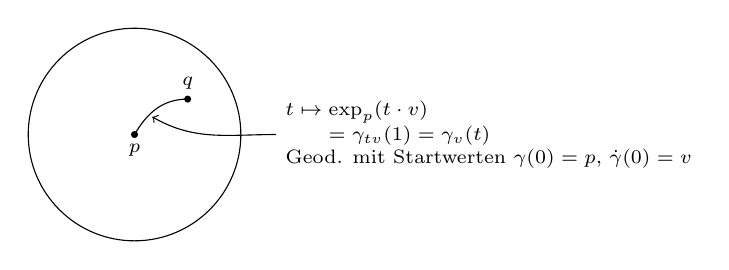
\begin{tikzpicture}[font=\scriptsize,scale=0.9]
      \coordinate (p) at (0,0); \coordinate (q) at (0.75,0.5);
      
      \draw[] (p) circle(1.5);
      \draw (p) to[out=60,in=180] (q);
      \fill (p) circle(0.05) node[below]{$p$} (q) circle(0.05) node[above]{$q$};
      
      \node[align=left] (txt) at (5,0) {$t \mapsto \exp_p(t \cdot v)$\\$\textcolor{white!100}{t \mapsto} = \gamma_{tv}(1) = \gamma_v(t)$\\Geod. mit Startwerten $\gamma(0)=p$, $\dot\gamma(0)=v$};
      \draw[->] (txt) to[out=180,in=330] (0.25,0.25);
    \end{tikzpicture}\end{center}
\end{Satz}

\begin{bew}
  \marginnote{\begin{tikzpicture}[font=\scriptsize,scale=0.7]
      %	\draw[step=0.25,gray!15] (-6,-3) grid (6,3); \draw[step=0.5,gray!30] (-6,-3) grid (6,3); \fill (0,0) circle(0.1); %Hilfsgitter
      \coordinate (p) at (0,0); \coordinate (q) at (3.25,1.5);
      \coordinate (a) at (1.5,1);
      \coordinate (ctrlp) at (0.25,1.5); \coordinate (ctrla) at (0.75,0.25); \coordinate (ctrlq) at (-1.75,1);
      \draw[dashed] (p) circle(1.75);
      \draw[name path=kreis] (p) circle(1);
      \draw[name path=kurve] (p) ..controls($(p) + (ctrlp)$) and ($(a) - (ctrla)$).. (a) ..controls($(a) + (ctrla)$) and ($(q) + (ctrlq)$).. (q) node[pos=0.6,above]{$c$};
      \begin{scope}
        \path[clip] (p) circle(1);
        \draw[very thick] (p) ..controls($(p) + (ctrlp)$) and ($(a) - (ctrla)$).. (a) ..controls($(a) + (ctrla)$) and ($(q) + (ctrlq)$).. (q);
      \end{scope}
      \fill (p) circle(0.1)node[below left]{$p$} (q) circle(0.1)node[above]{$q$};
      \draw[name path=strich] (p) -- (q);
      \path[name intersections={of={kreis and kurve}}];
      \coordinate (ct0) at (intersection-1);
      \path[name intersections={of={kreis and strich}}];
      \coordinate (q') at (intersection-1);
      \fill (ct0) circle(0.1)node[above]{$c(t_0)$} (q') circle(0.1)node[below right]{$q'$};
    \end{tikzpicture}}
  Es sei $\epsilon > 0$ so, dass auf $\B_{\epsilon}(p)$ Polorkoordinaten $\phi = (r,\theta^1, \ldots, \theta^{m-1})$ existieren.
  Sei weiter $c \colon [0,1] \to M$ eine beliebige glatte Kurve von $p$ nach $q$ mit Koordinaten $\phi(c(t)) = (r(t), \theta^1(t), \ldots, \theta^{m-1}(t))$.
  \begin{center}\begin{tikzpicture}[font=\scriptsize]
      %	\draw[step=0.25,gray!15] (-6,-6) grid (6,6); \draw[step=0.5,gray!30] (-6,-6) grid (6,6); \fill (0,0) circle(0.1); %Hilfsgitter
      
      \coordinate (segel) at (-3,-1);
      \tikzsegel[2]{(segel)};
      \coordinate (p) at ($(segel) + (2.5,1.25)$); \coordinate (q) at ($(segel) + (3.25,0.75)$);
      \coordinate (pkt1) at ($(segel) + (3.25,2)$); \coordinate (pkt2) at ($(segel) + (3.75,1.75)$);
      \coordinate (ctrl1) at (1,0); \coordinate (ctrl2) at (1,1); \coordinate (ctrl3) at (0,1); \coordinate (ctrl4) at (-1,-0.25);

      \fill (p) circle(0.05)node[left]{$p$}; \fill (q) circle(0.05)node[right]{$q$};
      \draw (p) ..controls($(p) + 0.75*(ctrl1)$) and ($(pkt1) - 0.25*(ctrl2)$).. (pkt1) ..controls($(pkt1) + 0.25*(ctrl2)$) and($(pkt2) + 0.25*(ctrl3)$).. (pkt2)node[right]{$c$} ..controls($(pkt2) - 0.5*(ctrl3)$) and($(q) + (ctrl4)$).. (q);
      
      \draw[clip] ($(segel) + (2.825,1)$) ellipse(1 and 0.5);
      \draw[very thick] (p) ..controls($(p) + 0.75*(ctrl1)$) and ($(pkt1) - 0.25*(ctrl2)$).. (pkt1);
    \end{tikzpicture}\\
    Das Bild von $c$ ist nicht notwendig in $\B_\epsilon(0)$ enthalten
  \end{center}
  F"ur $t_0 = \inf\{t \in [0,1] \mid c(t) \notin \B_{\epsilon}(p)\}$ ist $c|_{[0,t_0]}$ eine Kurve zu $\B_{\epsilon}(p)$.
  Es gilt
  \begin{align*}
    \left\|\pdifffrac[t]{}{r}\right\| = \|\dot\gamma_w(t)\| = \|w\| = 1.
  \end{align*}
  Aus der Cauchy-Schwarz-Ungleichung folgt
  \begin{align*}
    \|\dot c(t)\| & = \|\dot c(t)\|\left\|\pdifffrac[c(t)]{}{r}\right\|\\
    & \geq \left|\left< \dot c(t), \pdifffrac[c(t)]{}{r}\right>\right|\\
    & = \left|\left<\dot r(t) \pdifffrac{}{r} + \sum_{i=1}^{m-1}\dot\theta^i(t)\pdifffrac{}{\theta^i},\pdifffrac[c(t)]{}{r}\right>\right|\\
    & = \left|\left<\dot r(t)\pdifffrac[c(t)]{}{r}, \pdifffrac[c(t)]{}{r}\right>\right|\\
    & = \left|\dot r(t)\right|,
  \end{align*}
  wobei die Gleichheit genau dann gilt, wenn $\dot c(t)$ und $\pdifffrac[c(t)]{}{r}$ linear abh"angig sind.
  \begin{align*}
    \mathcal L(c) = \int_0^{t_0}\|\dot c\| + \int_{t_0}^T\|\dot c\| \geq \int_0^{t_0} \left|\left<\dot c,\pdifffrac{}{r}\right>\right| = \int_0^{t_0}|\dot r| = r(t_0)
  \end{align*}
  Gleichheit gilt genau dann, wenn $\theta^1(t), \ldots, \theta^{m-1}(t)$ konstant sind und $\dot r(t) \geq 0$ gilt, also genau dann, wenn $c$ eine monotone Umparametrisierung von $t \mapsto \exp_p(tv)$ f"ur $v \in S^{m-1}$ ist.

  F"ur den zweiten Teil sei $\epsilon$ so, dass Polarkoordinaten $\phi=(r, \theta^1,\ldots ,\theta^{m-1})$ um $p$ existieren.
  Es sei $q \in \B_\delta(p)$ und $c$ sei eine glatte Kurve von $p$ nach $q$.
  F"ur $t_0 = \inf \{ t \in [0,1] | c(t) \notin \B_\delta(p) \}$ gilt dann:
  \begin{align*}
    \calL(c) \ge \delta + \dop(c(t_0), q) \ge \delta + \dop(\partial \B_\delta(p), q),
  \end{align*}
  also $d(p,q) = \inf_c \calL(c) \ge \delta + \dop(\partial \B_\delta(p), q)$. Da $\partial \B_\delta(p)$ kompakt ist, die Abstandsfunktion $\dop(\cdot, q)$ auf $\partial \B_\delta(p)$ ihr Minimum in $q'$ an. Damit gilt
  \begin{align*}
    \dop(q',q) &= \dop(\partial \B_\delta(p), q) \qquad \text{und}\\
    \dop(p,q) &= \dop(p,q') + \dop(q',q) = \delta + \dop(q',q)
  \end{align*}
  somit gilt dann die Behauptung.
\end{bew}

\begin{Kor}\label{kor-8-8}
  F"ur alle $p \in M$ existiert ein $\rho > 0$, so dass f"ur alle $q, q' \in \B_\rho(p)$ genau eine minimierende Geod"atische von $q$ nach $q'$ existiert.
\end{Kor}

\begin{bew}
  F"ur $q \in M$ existiert ein $\rho = \rho(q) > 0$, so dass $\exp$ auf $\B_\rho(q)$ ein Diffeomorphismus ist.
  Da $\exp: \calD \to \calD$ glatt und $\calD$ offen ist, existiert eine Umgebung $U_q$ von $q$, so dass $\exp_p: \B_{\frac{\rho}{2}}(0_q) \to \B_{\frac{\rho}{2}}(q')$ ein Diffeomorphismus ist f"ur alle $q' \in U_q$.
  F"ur $p \in M$ existiert nach Satz \ref{satz-8-7} ein $\epsilon > 0$, so dass $\overline \B_\epsilon(p)$ kompakt ist.
  Die "Uberdeckung $\bigcup_{q \in \overline \B_\epsilon(q)} \B_{\frac{\rho(q)}{2}}(q)$ besitzt eine endliche Teil"uberdeckung.
  F"ur $\rho = \min_{i \le k} \{ \frac{\rho(q_i)}{4} \}$ existieren auf jedem $\B_{2\rho}(q)$, $q \in \B_\epsilon(p)$, Polarkoordinaten; insbesondere existiert f"ur $q, q' \in \B_\rho(p)$ eine eindeutige minimierende Geod"atische von $q$ nach $q'$.
\end{bew}

\begin{bem}
  Die Geod"atischen im obigen Korollar h"angen stetig von ihren Endpunkten ab.
\end{bem}

\begin{Kor}\label{kor-8-9}
  Es seien $p, q \in M$ und $c: [0,1] \to M$ st"uckweise glatte Kurven von $p$ nach $q$, so dass $\calL(c) = \dop(p,q)$.
  Damit ist $c$ eine umparametrisierte Geod"atische im Sinne von Definition \ref{dfn-8-1}.
\end{Kor}

\begin{bew}
  \marginnote{\begin{tikzpicture}[font=\scriptsize,scale=0.5]
      %	\draw[step=0.25,gray!15] (-6,-1) grid (6,5); \draw[step=0.5,gray!30] (-6,-1) grid (6,5); \fill (0,0) circle(0.1); %Hilfsgitter
      \draw[name path=kurve] (-3,0) ..controls(-3,0) and (-2.5,1).. (-1,1.5)node[above]{$c$} ..controls(0.5,2) and (2.5,2).. (2.5,2);
      \path[name path=links] (-2.5,0) -- (-2.5,3); \path[name path=right] (1,0) -- (1,3);
      \path[name intersections={of={kurve and links}}]; \coordinate (cs) at (intersection-1);
      \path[name intersections={of={kurve and right}}]; \coordinate (ct) at (intersection-1);
      \fill (cs) circle(0.1); \fill (ct) circle(0.1);
      \draw (cs)node[left]{$c(s)$} --node[below]{$\overline c$} (ct)node[above]{$c(t)$};
    \end{tikzpicture}}
  Die Kurve ist lokal l"angenminimierend, denn ist $\overline c$ eine Kurve von $c(s)$ nach $c(t)$ mit $\calL(\overline c) < \calL(c|_{[s,t]})$, so w"are $c|_{[0,s]} \cup \overline c \cup c|_{[t,1]}$ eine Kurve k"urzer als $c$.
  Da $c$ kompaktes Bild hat, exisitert ein minimales $\rho > 0$ f"ur alle $c(t)$ wie in Korollar \ref{kor-8-8}. Dann findet man eine Partition $0 = t_0 < t_1 < \ldots < t_k = 1$ mit $\dop(c(t_{i-1}), c(t_{i})) < \frac{\rho}{2}$, so dass $c|_{[t_{i-1}, t_{i+1}]}$ glatt ist.
  \begin{center}\begin{tikzpicture}[font=\scriptsize]
      %	\draw[step=0.25,gray!15] (-6,-5) grid (6,5); \draw[step=0.5,gray!30] (-6,-5) grid (6,5); \fill (0,0) circle(0.1); %Hilfsgitter
      
      \draw[dashed] (0,0) circle(1.5);
      \begin{scope}
        \path[name path=kreis,clip] (0,0) circle (1.0);
        \draw[very thick] (-2.5,-1) ..controls(-2.5,-1) and (-0.75,-0.5).. (0,0) ..controls(0.75,0.5) and (1.5,2).. (1.5,2);
      \end{scope}
      
      \draw[name path=kurve] (-2.5,-1) ..controls(-2.5,-1) and (-0.75,-0.5).. (0,0)node[right]{$c(t_i)$} ..controls(0.75,0.5) and (1.5,2).. (1.5,2) node[right,pos=0.7]{$c$};
      
      \path[name intersections={of={kreis and kurve}}];
      \fill (intersection-2) circle(0.05) node[right]{$c(t_{i-1})$}; \fill (intersection-1) circle(0.05) node[right]{$c(t_{i+1})$}; \fill (0,0) circle(0.05);
    \end{tikzpicture}\end{center}
  Dann stimmt $c|_{[t_{i-1}, t_{i+1}]}$ f"ur jedes $i < k$ mit der nach Korollar \ref{kor-8-8} eindeutigen Geod"atischen (bis auf Umparametrisierung) "uberein.
\end{bew}

\begin{Dfn}
  Eine Riemannsche Mannigfaltigkeit hei"st \CmMark[vollst\"andig!geo\"atisch]{geod"atisch vollst"andig}, wenn jede Geod"atische auf ganz $\R$ fortgesetzt werden kann.
\end{Dfn}

\begin{Satz}[Satz von Hopf-Rinow]\label{satz-8-11}\label{hopf-rinow}
  F"ur eine Riemannsche Mannigfaltigkeit sind die folgenden Aussagen "aquivalent:
  \begin{enumerate}[label=(\roman*),widest=iii]
  \item $M$ ist geod"atisch vollst"andig, das hei"st jede Geod"atische existiert f"ur alle Zeiten.
  \item F"ur alle $p \in M$ gilt $\calD_p = \T_pM$, also $\exp$ ist auf ganz $M$ definiert.
  \item Es existiert ein $p \in M$ mit $\calD_p = \T_pM$, also $\exp_p$ ist auf $\T_pM$ f"ur ein $p \in M$ definiert.
  \item Abgeschlossene und beschr"ankte Teilmengen sind kompakt.
  \item $M$ ist vollst"andig (als metrischer Raum).
  \end{enumerate}
  Jede dieser Eigenschaften impliziert, dass je zwei Punkte $p, q$ in $M$ durch eine minimierende Geod"atische von $p$ nach $q$ verbunden werden k"onnen.
\end{Satz}

\begin{bew}
  Man zeigt zun"achst, dass es, falls (iii) f"ur $p \in M$ gilt, zu jedem  $q \in M$ eine minimierende Geod"atische von $p$ nach $q$ gibt.
  Es gelte $\calD_p = \T_pM$ und es sei $q \in M$.
  \begin{center}\begin{tikzpicture}
      %	\draw[step=0.25,gray!15] (-6,-1) grid (6,5); \draw[step=0.5,gray!30] (-6,-1) grid (6,5); \fill (0,0) circle(0.1); %Hilfsgitter

      \draw (-2,4.5) -- (-3,2.5) -- (2,2.5);
      \coordinate (0p) at (-1.75,3.25);
      \fill(0p) circle(0.05) node[below left]{$0_p$}; \draw[->] (0p) -- +(1.5,0.75);
      
      \coordinate (p) at ($(0p) - (0,3.25)$); \coordinate (q) at ($(p) + (7,3)$);
      \fill (p) circle(0.05)node[left]{$p$} (q) circle(0.05)node[right]{$q$};
      \draw[dashed,name path=strich] (p) -- (q);
      
      \draw[name path=kreis] (p) circle(1.25);
      \path[name intersections={of={strich and kreis}}];
      \fill (intersection-1) circle(0.05) node[above]{$\overline q$};
      \draw[->] (p) -- (intersection-1);

    \end{tikzpicture}\end{center}
  F"ur $\epsilon > 0$ wie in Satz \ref{satz-8-7} ist $\partial \B_{\frac{\epsilon}{2}}(p)$ kompakt; es sei $\overline q \in \partial \B_{\frac{\epsilon}{2}}(p)$ ein Punkt minimalen Abstandes zu $q$.
  Dann gilt $\overline q = \exp_p(\frac{\epsilon}{2}v)$ f"ur ein $v \in \T_pM$ mit $\|v\| = 1$.
  \begin{description}[font=\normalfont\itshape]
  \item[Behauptung:] Dann ist $\gamma_v|_{[0,R]}: t \mapsto \exp_p(tv)$ minimierende Geod"atische nach $q$ f"ur $R = \dop(p,q)$.
  \end{description}
  Es sei $\calI = \{t \in [0,R] \mid \dop(\gamma_v(t),q) = R - t\}$. Dann ist $\calI$ nichtleer und abgeschlossen, denn $t \mapsto \dop(\gamma_v(t),q) + t$ ist stetig.
  \begin{center}\begin{tikzpicture}[font=\scriptsize]
      %	\draw[step=0.25,gray!15] (-6,-1) grid (6,5); \draw[step=0.5,gray!30] (-6,-1) grid (6,5); \fill (0,0) circle(0.1); %Hilfsgitter
      
      \coordinate (p) at (-3,0); \coordinate (p0) at (3.5,2.5);
      \coordinate(ctrlp) at (0.5,1.5); \coordinate(ctrlp0) at (-2.5,-0.25);
      \coordinate (q) at ($(p0) - 1.25*(ctrlp0)$);
      
      \draw (p) ..controls($(p) + (ctrlp)$) and ($(p0) + (ctrlp0)$)..node[below]{$\gamma_v$} (p0);
      \fill (p) circle(0.05) node[below]{$p$} (p0) circle(0.05) node[below]{$p_0= \gamma_v(t_0)$} (q) circle(0.05) node[right]{$q$};

      \path[name path=strich] (p0) -- (q);
      
      \draw[dashed,name path=kreis] (p0) circle(1.25);
      
      \path[name intersections={of={kreis and strich}}];
      \draw (p0) -- (intersection-1); \draw[dashed] (intersection-1) -- (q);
      \fill (intersection-1) circle(0.05) node[below right]{$q'$};
    \end{tikzpicture}\end{center}
  F"ur $t_0 \in \calI$ und $0 < \rho < \epsilon_0$ sei $q' \in \partial \B_\rho(\gamma_v(t_0))$ wie in Satz \ref{satz-8-7} angewandt auf $p_0 = \gamma_v(t_0)$. Dann gilt $\dop(p_0, q) = \rho + \dop(q',q)$ und es folgt:
  \begin{align*}
    \dop(p,q') &\ge \dop(p,q) - \dop (q',q)\\
    &= \dop(p,q) - \dop(p_0,q) + \rho\\
    &= R - (R - t) + \rho = t_0 + \rho
  \end{align*}
  Damit ist die Verkettung von $\gamma_v|_{[0,t_v]}$ und der minimalen Geod"atischen von $p_0$ nach $q'$ nach Korollar \ref{kor-8-9} eine Geod"atische.
  Aus der Eindeutigkeit von kurzen Geod"atischen folgt, dass diese Zusamensetzung mit $\gamma_v$ "ubereinstimmt.
  Es gilt also $q' = \gamma_v(t_0 + \rho)$ und mit $\dop(\gamma_v(t_0 + \rho), q) = \dop(p_0,q) - \rho = R - (t_0 + \rho)$ gilt $t_0 + \rho \in \calI$.

  Wir k"onnen nun die einzelnen Implikationen zeigen.
  Dabei gelten (i) $\Rightarrow$ (ii) $\Rightarrow$ (iii) offensichtlich.
  \begin{description}[font=\normalfont]
  \item[(iii) $\Rightarrow$ (iv):]
    Es gelte $\calD_p = \T_pM$ und es sei $K \subseteq M$ abgeschlossen und beschr"ankt.
    Dann existiert $R$ mit $K \subseteq \overline\B_R(p)$. Da $\overline\B_R(0_p)$ kompakt ist, ist auch $K$ kompakt.
  \item[(iv) $\Rightarrow$ (v):]
    gilt offensichtlich
  \item[(v) $\Rightarrow$ (i):]
    Es sei $c$ eine nach Bogenl"ange parametrisierte Geod"atische mit maximalem Definitionsintervall $\calI$. $\calI$ ist nichtleer und offen.
    Ist $(t_n)$ eine Folge in $\calI$ mit Grenzwert $t$.
    Dann ist $q_n = c(t_n)$ wegen
    \[ \dop(c(t_n), c(t_m)) \le |t_m - t_n| \]
    eine Cauchy-Folge und konvergiert somit gegen ein $p \in M$.
    \begin{center}
      \begin{tikzpicture}[font=\scriptsize,scale=0.9]
% \draw[step=0.25,gray!15] (-6,-3) grid (6,3); \draw[step=0.5,gray!30] (-6,-3) grid (6,3); \fill (0,0) circle(0.1); %Hilfsgitter
        
\coordinate (ctn) at (0,0);
\coordinate (ctrl) at (0,1); 
        
% ich muss an ddieser Stelle schummeln, auskommentiert ist der richtige Code, aber das Kompilieren dauert zu lange mit Fixed Point Arithmetic -Aleks

\draw[clip] (ctn) circle(2);
\draw[dashed] (ctn) circle(1);
% \draw[fixed point arithmetic,decoration={markings, mark=at position 0.8 with {\arrow{>};}},postaction={decoration={markings, mark=at position 0.2 with {\arrow{>};}},decorate}] (-1,-2.5) .. controls(-1,-2.5) and ($(ctn) - (ctrl)$).. node[right,pos=0.6]{$c$} (ctn) ..controls($(ctn) + (ctrl)$) and (-0.5,2.5).. (-0.5,2.5);

\draw (-1,-2.5) .. controls(-1,-2.5) and ($(ctn) - (ctrl)$).. node[right,pos=0.6]{$c$}node[sloped]{>} (ctn) ..controls($(ctn) + (ctrl)$) and (-0.5,2.5)..node[sloped]{<} (-0.5,2.5);

\filldraw[fill=white] (ctn) circle(0.06)node[above right]{$p$};
\fill ($(ctn) - (0.02,0.3)$) circle(0.05)node[right]{$c(t_n)$};

\end{tikzpicture}
    \end{center}
    Es sei $\rho > 0$ wie in Korollar \ref{kor-8-8}. F"ur hinreichend gro"ses $n$ gilt dann $|t_n - t| < \frac{\rho}{2}$. Die nach Bogenl"ange parametrisierte Geod"atische von $q_n = c(t_n)$ mit Startvektor $\dot c(t_n)$ existiert auf $(-\frac{\rho}{2}, \frac{\rho}{2})$, setzt also $c$ bis zum Zeitpunkt $|t_n| + \frac{\rho}{2} > |t|$ fort.
  \end{description}
\end{bew}

%% 
%% Vorlesung <2013-1-8 Tue>
%% 

\begin{emptythm}[Bemerkungen/Beispiele]
  \begin{enumerate}[label=(\arabic*),leftmargin=*]
  \item Geod"atische sind im Allgemeinen nicht eindeutig. Betrachte die Einheitssph"are mit Geod"atischen vom Nord- zum S"udpol:
    \begin{center}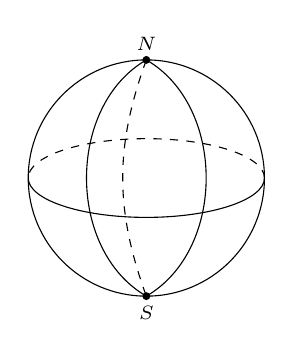
\begin{tikzpicture}[font=\scriptsize]
        \draw (0,0) circle(1.5);
        \begin{scope}
          \clip (-1.5,0) rectangle (1.5,-1);
          \draw (0,0) ellipse(1.5 and 0.5);
        \end{scope}\begin{scope}
          \clip (-1.5,0) rectangle (1.5,1);
          \draw[dashed] (0,0) ellipse(1.5 and 0.5);
        \end{scope}
        
        \coordinate (N) at (0,1.5); \coordinate (S) at (0,-1.5);
        \fill (N) circle (0.05) node[above]{$N$} (S) circle (0.05) node[below]{$S$};
        
        \draw (N) to[out=330,in=30] (S);
        \draw (N) to[out=210,in=150] (S);
        \draw[dashed] (N) to[out=250,in=110] (S);
      \end{tikzpicture}\end{center}
  \item $\R^2 \setminus \{0\}$
    \begin{center}\begin{tikzpicture}[font=\scriptsize,scale=2]
        \draw[->] (-1.5,0) -- (1.5,0);
        \draw[->] (0,-0.5) -- (0,1);
        \filldraw[fill=white] (0,0) circle(0.05);
        \draw (-1,0.1) -- (-1,-0.1)node[below]{$-1$} (1,0.1) -- (1,-0.1)node[below]{$1$};
        
        \def\faktor{0.1}
        \def\tangente{0.5}
        \foreach \y in {1, 2, 3, 4}{
          \coordinate (cntr) at ($(0,0) + \faktor*(0,\y)$);
          \draw (-1,0) ..controls(-1,0) and ($(cntr) - \tangente*(1,0)$).. (cntr) ..controls($(cntr) + \tangente*(1,0)$) and (1,0).. (1,0);
        }
      \end{tikzpicture}\end{center}
  \item $\B_1(0) \subseteq \R^2$ ist geod"atisch konvex aber nicht vollst"andig.
  \end{enumerate}
\end{emptythm}

\begin{Kor}\label{thm:kor-8-12}
  Es seien $M$ eine vollst"andige Riemannsche Mannigfaltigkeit und $c$ eine Geod"atische. Dann gilt:
  \begin{enumerate}[label=(\roman*),widest=iii,leftmargin=*]
  \item $c$ ist lokal l"angenminimierend.
  \item Falls es keine k"urzere Geod"atische von $c(a)$ nach $c(b)$ gibt, so ist $c|_{[a,b]}$ minimal.
  \item Falls es eine weitere Geod"atische $\overline{c}$ von $c(a)$ nach $c(b)$ mit $\calL(\overline c) = \calL(c|_{[a,b]})$ gibt, so ist $c|_{[a,b+\epsilon]}$ f"ur kein $\epsilon$ minimierend.\label{thm:kor-8-12-iii} 
  \end{enumerate}
\end{Kor}

\begin{bew}
  \begin{enumerate}[label=(\roman*),widest=iii,leftmargin=*]
  \item Siehe Korollar \ref{kor-8-9}.
  \item Nach dem Satz von Hopf-Rinow existiert eine minimale Geod"atische von $c(a)$ nach $c(b)$. Ist $c$ also die K"urzeste von $c(a)$ nach $c(b)$, so ist $c$ auch minimierend.
  \item Ist $\overline c$ eine weitere Geod"atische von $c(a)$ nach $c(b)$, so gilt $\dot c(b) \ne \dot{\overline{c}}(b)$.
    \begin{center}
      \begin{tikzpicture}[font=\scriptsize, tangent/.style={
          decoration={
            markings,% switch on markings
            mark=
            at position #1
            with
            {
              \coordinate (tangent point-\pgfkeysvalueof{/pgf/decoration/mark info/sequence number}) at (0pt,0pt);
              \coordinate (tangent unit vector-\pgfkeysvalueof{/pgf/decoration/mark info/sequence number}) at (1,0pt);
              \coordinate (tangent orthogonal unit vector-\pgfkeysvalueof{/pgf/decoration/mark info/sequence number}) at (0pt,1);
            }
          },
          postaction=decorate
        },
        use tangent/.style={
          shift=(tangent point-#1),
          x=(tangent unit vector-#1),
          y=(tangent orthogonal unit vector-#1)
        },
        use tangent/.default=1]
        % \tikzgitter{(-5,-5)}{(5,5)}
        
        \coordinate (a) at (-3,-2); \coordinate (ende) at (3,3);
        \coordinate (ctrla1) at (2,0.25); \coordinate (ctrlende) at (-0.5,-3); \coordinate (ctrlende) at (-0.5,-2.75);
        \fill (a) circle(0.05)node[below]{$c(a)$};
        
        % Zeichen die Kurve und definiere den Punkt b auf der Kurve
        \draw[tangent=0.8] (a) ..controls($(a) + (ctrla1)$) and ($(ende) + (ctrlende)$).. coordinate[pos=0.8] (b) coordinate[pos=0.95] (d) (ende);
        \draw[->,use tangent] (0,0) -- (1,0)node[below right]{$\dot c(b)$};
        \fill (b) circle(0.05)node[below,xshift=2mm]{$c(b)$};
        \draw[dashed] (b) circle (1.5);
        
        \coordinate (ctrla2) at (1,2.5); \coordinate (ctrlb) at (-1.5,0);
        \draw[tangent=1] (a) ..controls($(a) + (ctrla2)$) and ($(b) + (ctrlb)$)..node[above left]{$\overline c$} coordinate[pos=0.75] (e) (b);
        \draw[->,use tangent] (0,0) -- (1,0)node[below]{$\dot{\overline c}(b)$};
        
        \fill (d) circle(0.05) (e) circle(0.05);
        
        \begin{scope}
          \clip (b) rectangle (d);
          \draw[very thick] (a) ..controls($(a) + (ctrla1)$) and ($(ende) + (ctrlende)$).. (ende);
        \end{scope}\begin{scope}
          \clip ($(b)+(0,1)$) rectangle ($(e) - (0,1)$);
          \draw[very thick] (a) ..controls($(a) + (ctrla2)$) and ($(b) + (ctrlb)$)..(b);
        \end{scope}
        
        \draw (e) ..controls(2,1.5) and (2.5,2)..node[above left]{$\tilde c$} (d);
      \end{tikzpicture}\\
      \scriptsize{Die zusammengesetzte Kurve kann keine Geod"atische sein, da die Tangentialvektoren nicht "ubereinstimmen.}\end{center}
    F"ur hinreichend kleines $\epsilon > 0$ existiert dann nach Satz \ref{satz-8-7} eine minimierende Geod"atische $\tilde c$ von $\overline c(b-\epsilon)$ nach $c(b+\epsilon)$.
    Die L"ange von $\overline c|_{[a,b-\epsilon]} \cup \tilde c$ ist strikt kleiner als die L"ange von $c|_{[a,b+\epsilon]}$.
    Damit ist $c|_{[a,b+\epsilon]}$ nicht minimierend.
  \end{enumerate}
\end{bew}

%%% Local Variables: 
%%% mode: latex
%%% TeX-master: "../skript-diffgeom"
%%% End: 
